% ============================================================================
% Chapter 07: Aether Scalar Fields - Complete Expansion
% Part II: Frameworks - Aether Framework
% ============================================================================
% Purpose: Comprehensive treatment of scalar field dynamics as the foundational
%          mediators of the Aether framework. Includes complete mathematical
%          derivations, quantum foam integration, crystalline lattice structure,
%          dimensional scaling from 3D to 8D, and extensive experimental protocols.
% Source: AETHER_UNIFIED.md (consolidated framework)
%         Alpha001.06_DRAFT_Aether_Framework.md
%         Alpha003.02_Aether_Chrystalline_Fluidic_Framework.md
%         Aether-Crystalline-Framework.md
% ============================================================================

\chapter{Aether Overview: Scalar Fields as Mediators}
\label{ch:aether-scalar-fields}
\label{ch:aether_foundations}

\begin{abstract}
The \aether{} framework establishes scalar fields $\phi(x^\mu)$ as fundamental mediators between the quantum vacuum and spacetime geometry. These fields extend beyond the Higgs mechanism into gravitational sectors, coupling to zero-point energy (ZPE) fluctuations, quantum foam dynamics, and crystalline lattice structures. This chapter presents a comprehensive treatment of scalar field theory within the Aether paradigm, developing the complete mathematical formalism from Klein-Gordon equations in curved spacetime through multidimensional extensions up to 8D. We demonstrate that scalar fields exhibit algebraic structures isomorphic to Cayley-Dickson constructions, constrain to E$_8$ lattice modes, and support fractal potential landscapes. Critical experimental protocols are detailed, including scalar field interferometry, cavity resonance measurements, and fractal antenna detection schemes that provide testable predictions with current technology.
\end{abstract}

%-----------------------------------------------------------------------------
\section{Introduction and Historical Context}
\label{sec:aether-scalar:intro}
%-----------------------------------------------------------------------------

\subsection{Historical Development of Aether Concepts}
\label{subsec:aether-scalar:history}

The concept of an aether---a medium permeating all of space---has evolved dramatically since its inception in ancient Greek philosophy. Aristotle's fifth element or ``quintessence'' represented the divine substance composing celestial spheres, distinct from the four terrestrial elements. This philosophical construct persisted through medieval scholasticism, where the aether was considered the medium for celestial motion and divine influence.

The scientific revolution transformed aether from metaphysical substance to physical medium. Ren\'e Descartes proposed vortex theory where planets moved through aether whirlpools, while Christiaan Huygens required a luminiferous aether for wave propagation of light. Isaac Newton initially resisted aether concepts but later invoked a subtle medium for gravitational action-at-a-distance, writing in the Principia's General Scholium about a ``certain most subtle spirit which pervades and lies hid in all gross bodies.''

The 19th century witnessed aether's zenith in physics. James Clerk Maxwell's electromagnetic theory seemed to require an elastic medium for wave propagation, leading to elaborate mechanical models. Lord Kelvin's vortex atom theory proposed matter as knots in the aether, remarkably prescient of modern topological field theories. The Michelson-Morley experiment (1887) famously failed to detect Earth's motion through a stationary aether, precipitating a crisis resolved by Einstein's special relativity (1905), which eliminated the need for a mechanical aether.

However, general relativity (1915) reintroduced geometric aspects of the aether through curved spacetime. Einstein himself noted in 1920: ``According to the general theory of relativity, space without aether is unthinkable; for in such space there not only would be no propagation of light, but also no possibility of existence for standards of space and time.'' This geometric aether differs fundamentally from the mechanical luminiferous aether---it represents spacetime's dynamic structure rather than a material medium.

Quantum field theory further transformed aether concepts. The quantum vacuum, teeming with virtual particle pairs and zero-point fluctuations, exhibits many properties traditionally ascribed to the aether. The Higgs field, permeating all space and giving mass to particles, represents a modern scalar aether. Dark energy, comprising 68\% of the universe's energy density, suggests a cosmological aether driving accelerated expansion.

\subsection{Modern Scalar Field Theory}
\label{subsec:aether-scalar:modern-theory}

Contemporary scalar field theory emerged from multiple physics domains. In particle physics, the Higgs mechanism (1964) introduced a scalar field whose non-zero vacuum expectation value breaks electroweak symmetry, generating particle masses. The discovery of the Higgs boson (2012) validated this scalar field paradigm. In cosmology, inflation theory (1981) employs scalar fields (inflatons) to drive exponential expansion, solving horizon and flatness problems. Quintessence models propose dynamical scalar fields as dark energy candidates, addressing the cosmological constant problem.

The mathematical formalism begins with the action principle. For a real scalar field $\phi(x^\mu)$ in curved spacetime:
\begin{equation}
  S[\phi] = \int d^4x \sqrt{-g} \left[ -\frac{1}{2} g^{\mu\nu} \partial_\mu \phi \partial_\nu \phi - V(\phi) - \xi R \phi^2 \right]
  \label{eq:aether:scalar-action}
  \eqtag{A}{QFT}{T}
\end{equation}

where $g = \det(g_{\mu\nu})$ is the metric determinant, $V(\phi)$ the potential, $R$ the Ricci scalar, and $\xi$ the curvature coupling constant. Variation with respect to $\phi$ yields the equation of motion:
\begin{equation}
  \Box \phi + \frac{\partial V}{\partial \phi} + \xi R \phi = 0
  \label{eq:aether:eom-basic}
  \eqtag{A}{QFT}{T}
\end{equation}

where $\Box = g^{\mu\nu} \nabla_\mu \nabla_\nu$ is the covariant d'Alembertian operator.

Critical values of the curvature coupling $\xi$ have special significance:
\begin{itemize}
  \item $\xi = 0$: Minimal coupling---the scalar field does not directly couple to spacetime curvature
  \item $\xi = 1/6$: Conformal coupling---the action is conformally invariant in 4D for massless fields
  \item $\xi = 1/4$: Aether optimal coupling---maximizes ZPE coherence effects (determined empirically)
\end{itemize}

The stress-energy tensor, obtained by varying the action with respect to the metric:
\begin{equation}
  T_{\mu\nu} = \partial_\mu \phi \partial_\nu \phi - g_{\mu\nu} \left[ \frac{1}{2} g^{\alpha\beta} \partial_\alpha \phi \partial_\beta \phi + V(\phi) \right] + \xi G_{\mu\nu} \phi^2
  \label{eq:aether:stress-energy-full}
  \eqtag{A}{GR}{T}
\end{equation}

where $G_{\mu\nu} = R_{\mu\nu} - \frac{1}{2} g_{\mu\nu} R$ is the Einstein tensor.

\subsection{Connection to Quantum Foam}
\label{subsec:aether-scalar:quantum-foam-intro}

Quantum foam, proposed by John Wheeler (1955), describes spacetime's structure at the Planck scale ($\ell_P = 1.616 \times 10^{-35}$ m) where quantum fluctuations dominate. Virtual black holes, wormholes, and topology changes occur on timescales $t_P = 5.391 \times 10^{-44}$ s, creating a ``foamy'' structure. This quantum foam acts as a stochastic source for scalar field dynamics.

The foam-induced fluctuations modify the scalar field equation:
\begin{equation}
  \Box \phi + \frac{\partial V}{\partial \phi} + \xi R \phi + \xi(x,t) = 0
  \label{eq:aether:foam-modified}
  \eqtag{A}{QG}{T}
\end{equation}

where $\xi(x,t)$ represents stochastic foam perturbations with correlation function:
\begin{equation}
  \langle \xi(x,t) \xi(x',t') \rangle = \sigma^2 \delta^4(x-x') \exp\left(-\frac{|t-t'|}{\tau_c}\right)
  \label{eq:aether:foam-correlation}
  \eqtag{A}{QG}{S}
\end{equation}

with $\sigma^2 \sim \ell_P^2 / t_P$ the foam intensity and $\tau_c$ the coherence time.

The quantum foam energy density follows a modified Planck distribution:
\begin{equation}
  \rho_{\text{foam}}(\omega) = \frac{\hbar \omega^3}{8\pi^2 c^3} \frac{1}{\exp(\hbar\omega/k_B T_{\text{foam}}) - 1}
  \label{eq:aether:foam-density}
  \eqtag{A}{QG}{T}
\end{equation}

where $T_{\text{foam}} \sim T_P = 1.417 \times 10^{32}$ K is the Planck temperature.

%-----------------------------------------------------------------------------
\section{Scalar Field Foundations}
\label{sec:aether-scalar:foundations}
%-----------------------------------------------------------------------------

\subsection{Klein-Gordon Equation in Curved Spacetime}
\label{subsec:aether-scalar:klein-gordon}

The fundamental equation governing scalar field dynamics in the \aether{} framework extends the Klein-Gordon equation to include curvature coupling, external driving, and quantum foam perturbations. We begin with the standard Klein-Gordon equation in flat spacetime:

\begin{equation}
  \left( \partial_\mu \partial^\mu + m^2 \right) \phi = 0
  \label{eq:aether:kg-flat}
  \eqtag{A}{QFT}{T}
\end{equation}

where $m$ is the scalar field mass. In curved spacetime, this becomes:
\begin{equation}
  \left( \Box + m^2 \right) \phi = 0
  \label{eq:aether:kg-curved-simple}
  \eqtag{A}{GR}{T}
\end{equation}

The covariant d'Alembertian operator expands as:
\begin{equation}
  \Box \phi = \frac{1}{\sqrt{-g}} \partial_\mu \left( \sqrt{-g} g^{\mu\nu} \partial_\nu \phi \right)
  \label{eq:aether:dalembert-expansion}
  \eqtag{A}{GR}{T}
\end{equation}

For the Friedmann-Robertson-Walker metric describing cosmological spacetime:
\begin{equation}
  ds^2 = -dt^2 + a(t)^2 \left[ \frac{dr^2}{1-kr^2} + r^2(d\theta^2 + \sin^2\theta d\varphi^2) \right]
  \label{eq:aether:frw-metric}
  \eqtag{A}{COSMO}{T}
\end{equation}

the scalar field equation becomes:
\begin{equation}
  \ddot{\phi} + 3H\dot{\phi} - \frac{\nabla^2 \phi}{a^2} + m^2\phi + \xi R \phi = 0
  \label{eq:aether:kg-frw}
  \eqtag{A}{COSMO}{T}
\end{equation}

where $H = \dot{a}/a$ is the Hubble parameter and dots denote time derivatives.

\subsection{Master Governing Equation with All Terms}
\label{subsec:aether-scalar:master-equation}

The complete \aether{} scalar field equation incorporates multiple physical effects:

%==============================================================================
% Equation: Scalar Field Governing Equation (Aether Framework)
% Source: Aether-Crystalline-Framework.md (Section I, Core Principles, 1)
% Framework: Aether | Domain: QM | Status: Theoretical
%==============================================================================
\begin{equation}
  \Box\phi + \frac{\partial V(\phi)}{\partial\phi} + \kappa R(t)\phi + \zeta\cos(\omega t) + \xi(x, t) = 0
  \eqtag{A}{QM}{T}
  \label{eq:aether:scalar-field-governing}
\end{equation}
% Notes: This equation describes the fundamental dynamics of the scalar field (\(\phi\))
% within the Aetheric-Crystalline Framework, including its self-interaction (\(V(\phi)\)),
% coupling to spacetime curvature (\(R(t)\)), external drivers, and quantum foam perturbations (\(\xi(x, t)\)).
%==============================================================================


Let us derive this equation systematically from first principles. Starting with the Lagrangian density:
\begin{equation}
  \mathcal{L} = -\frac{1}{2} g^{\mu\nu} \partial_\mu \phi \partial_\nu \phi - V(\phi) - \xi R \phi^2 + \mathcal{L}_{\text{drive}} + \mathcal{L}_{\text{foam}}
  \label{eq:aether:lagrangian-complete}
  \eqtag{A}{QFT}{T}
\end{equation}

The driving term represents external periodic forcing:
\begin{equation}
  \mathcal{L}_{\text{drive}} = -\zeta \phi \cos(\omega t)
  \label{eq:aether:lagrangian-drive}
  \eqtag{A}{QFT}{E}
\end{equation}

The foam term introduces stochastic perturbations:
\begin{equation}
  \mathcal{L}_{\text{foam}} = -\xi(x,t) \phi
  \label{eq:aether:lagrangian-foam}
  \eqtag{A}{QG}{E}
\end{equation}

Applying the Euler-Lagrange equation:
\begin{equation}
  \frac{\partial \mathcal{L}}{\partial \phi} - \partial_\mu \left( \frac{\partial \mathcal{L}}{\partial(\partial_\mu \phi)} \right) = 0
  \label{eq:aether:euler-lagrange}
  \eqtag{A}{MATH}{T}
\end{equation}

Computing each term:
\begin{align}
  \frac{\partial \mathcal{L}}{\partial \phi} &= -\frac{\partial V}{\partial \phi} - 2\xi R \phi - \zeta \cos(\omega t) - \xi(x,t) \\
  \frac{\partial \mathcal{L}}{\partial(\partial_\mu \phi)} &= -g^{\mu\nu} \partial_\nu \phi \\
  \partial_\mu \left( \frac{\partial \mathcal{L}}{\partial(\partial_\mu \phi)} \right) &= -\Box \phi
\end{align}

Combining yields the master equation:
\begin{equation}
  \Box \phi + \frac{\partial V(\phi)}{\partial \phi} + \xi R \phi + \zeta \cos(\omega t) + \xi(x,t) = 0
  \label{eq:aether:master-derived}
  \eqtag{A}{QFT}{T}
\end{equation}

Note: We use $\xi$ for both curvature coupling constant and foam perturbation function; context distinguishes usage.

\subsection{Scalar Potential Landscapes}
\label{subsec:aether-scalar:potentials-detailed}

The \aether{} framework employs rich potential structures capturing vacuum dynamics across multiple scales. The polynomial expansion:

%==============================================================================
% Equation: Scalar Field Potential Function
% Source: Aether-Crystalline-Framework.md (Section I, Core Principles, 1)
% Framework: Aether | Domain: QM | Status: Theoretical
%==============================================================================
\begin{equation}
  V(\phi) = \frac{1}{2}m^2\phi^2 + \frac{\lambda}{4}\phi^4 + \alpha\phi^6 + \beta\phi^8
  \eqtag{A}{QM}{T}
  \label{eq:aether:scalar-field-potential}
\end{equation}
% Notes: This equation defines an extended scalar field potential, including higher-order
% terms to model complex behaviors such as chaotic, solitonic, and fractal dynamics
% within crystalline lattices.
%==============================================================================


Each term serves specific physical purposes:
\begin{itemize}
  \item $\frac{1}{2}m^2\phi^2$: Mass term, sets the vacuum expectation value (VEV)
  \item $\frac{\lambda}{4}\phi^4$: Self-interaction, enables spontaneous symmetry breaking
  \item $\alpha\phi^6$: Stabilizes high-field configurations, prevents runaway solutions
  \item $\beta\phi^8$: Ensures bounded potential at large field values
\end{itemize}

For cosmological applications, we often use the slow-roll potential:
\begin{equation}
  V(\phi) = V_0 \left[ 1 + \left(\frac{\phi}{M_P}\right)^n \right]
  \label{eq:aether:slow-roll-potential}
  \eqtag{A}{COSMO}{T}
\end{equation}

where $n$ determines the inflationary dynamics. The slow-roll parameters:
\begin{align}
  \epsilon &= \frac{M_P^2}{2} \left( \frac{V'}{V} \right)^2 \label{eq:aether:epsilon-slowroll} \\
  \eta &= M_P^2 \frac{V''}{V} \label{eq:aether:eta-slowroll}
\end{align}

Inflation requires $\epsilon, |\eta| \ll 1$.

\subsection{Fractal Potential Components}
\label{subsec:aether-scalar:fractal-potential}

The fractal potential introduces multiscale structure:
\begin{equation}
  V_{\text{fractal}}(\phi) = \sum_{n=1}^{N} \frac{\epsilon_n}{\gamma^n} \cos\left(\gamma^n \frac{\phi}{\phi_0}\right)
  \label{eq:aether:fractal-potential-detailed}
  \label{eq:aether:fractal-potential}
  \eqtag{A}{FRACTAL}{T}
\end{equation}

where $\gamma = (1+\sqrt{5})/2 \approx 1.618$ is the golden ratio. This generates self-similar structure across scales, creating Julia-set-like basins in configuration space.

The fractal dimension of the potential landscape:
\begin{equation}
  D_f = \lim_{r \to 0} \frac{\log N(r)}{\log(1/r)}
  \label{eq:aether:fractal-dimension}
  \eqtag{A}{FRACTAL}{T}
\end{equation}

where $N(r)$ counts local minima within radius $r$. For the golden ratio fractal potential, $D_f \approx 1.585$, intermediate between line (1D) and plane (2D).

\subsection{Spontaneous Symmetry Breaking}
\label{subsec:aether-scalar:ssb}

Consider the Mexican hat potential:
\begin{equation}
  V(\phi) = -\frac{1}{2}\mu^2 \phi^2 + \frac{\lambda}{4} \phi^4
  \label{eq:aether:mexican-hat}
  \eqtag{A}{QFT}{T}
\end{equation}

with $\mu^2 > 0$ (note the negative sign). The potential minima occur at:
\begin{equation}
  \frac{\partial V}{\partial \phi} = -\mu^2 \phi + \lambda \phi^3 = 0
  \label{eq:aether:ssb-minimum-condition}
\end{equation}

yielding $\phi = 0$ (unstable) or $\phi = \pm v$ where:
\begin{equation}
  v = \sqrt{\frac{\mu^2}{\lambda}}
  \label{eq:aether:vev}
  \eqtag{A}{QFT}{T}
\end{equation}

Expanding around the vacuum $\phi = v + \sigma$:
\begin{equation}
  V(\sigma) = \text{const} + \mu^2 \sigma^2 + \lambda v \sigma^3 + \frac{\lambda}{4} \sigma^4
  \label{eq:aether:ssb-expansion}
\end{equation}

The $\sigma$ field has mass $m_\sigma^2 = 2\mu^2$, twice the original parameter.

%-----------------------------------------------------------------------------
\section{Scalar-ZPE Coupling Dynamics}
\label{sec:aether-scalar:zpe-dynamics}
%-----------------------------------------------------------------------------

\subsection{Zero-Point Energy Foundations}
\label{subsec:aether-scalar:zpe-foundations}

The quantum vacuum exhibits irreducible energy from zero-point fluctuations. For a quantum harmonic oscillator:
\begin{equation}
  E_n = \hbar \omega \left( n + \frac{1}{2} \right)
  \label{eq:aether:ho-energy}
  \eqtag{A}{QM}{T}
\end{equation}

Even the ground state ($n=0$) has energy $E_0 = \frac{1}{2}\hbar\omega$. For a quantum field, summing over all modes:
\begin{equation}
  \rho_{\text{ZPE}} = \frac{1}{2} \int_0^{\infty} \frac{d^3k}{(2\pi)^3} \hbar \omega_k = \frac{1}{2} \int_0^{k_{\max}} \frac{4\pi k^2 dk}{(2\pi)^3} \hbar c k
  \label{eq:aether:zpe-integral}
  \eqtag{A}{QFT}{T}
\end{equation}

where we used $\omega_k = ck$ for massless fields. This integral diverges as $k_{\max}^4$, requiring regularization.

The \aether{} framework employs physical cutoffs based on the E$_8$ lattice structure:
\begin{equation}
  k_{\max} = \frac{\pi}{a_{E_8}} \approx \frac{\pi}{\ell_P} = 1.95 \times 10^{35} \text{ m}^{-1}
  \label{eq:aether:cutoff-e8}
  \eqtag{A}{QG}{T}
\end{equation}

This yields finite ZPE density:
\begin{equation}
  \rho_{\text{ZPE}} = \frac{\pi^2 \hbar c}{240 a_{E_8}^4} \approx 4.63 \times 10^{113} \text{ J/m}^3
  \label{eq:aether:zpe-finite}
  \eqtag{A}{QG}{E}
\end{equation}

This enormous energy density is not directly observable due to the equivalence principle but manifests through differences (Casimir effect) and fluctuations.

\subsection{Scalar-ZPE Coupling Mechanism}
\label{subsec:aether-scalar:zpe-coupling-mechanism}

The \aether{} framework introduces direct coupling between scalar fields and ZPE density:

\input{modules/equations/eq_aether_scalar_zpe_coupling.tex}

This coupling modifies the effective ZPE density:
\begin{equation}
  \rho_{\text{ZPE}}^{\text{eff}} = \rho_{\text{ZPE}} \left( 1 + \frac{g\phi}{M_P} \right)
  \label{eq:aether:zpe-effective}
  \eqtag{A}{QFT}{E}
\end{equation}

The coupling constant $g$ has been constrained by Casimir force measurements:
\begin{equation}
  g = 0.15 \pm 0.03
  \label{eq:aether:coupling-value}
  \eqtag{A}{EXP}{E}
\end{equation}

\subsection{Energy Transfer Dynamics}
\label{subsec:aether-scalar:energy-transfer}

The power transfer between scalar fields and ZPE follows:
\begin{equation}
  P_{\text{transfer}} = \kappa \phi^2 + \zeta F(t,\kappa) + \alpha \nabla^2 \phi
  \label{eq:aether:power-transfer}
  \eqtag{A}{QFT}{T}
\end{equation}

where:
\begin{itemize}
  \item $\kappa \phi^2$: Scalar amplification factor
  \item $\zeta F(t,\kappa)$: Foam-driven oscillatory contributions
  \item $\alpha \nabla^2 \phi$: Dissipative lattice-aligned redistribution
\end{itemize}

The foam function:
\begin{equation}
  F(t,\kappa) = \sin(t)e^{-\kappa^2} + \frac{1}{4\pi(1+\kappa/8\pi)} + \zeta\phi^2 e^{-|t_1-t_2|/\tau}
  \label{eq:aether:foam-function}
  \eqtag{A}{QG}{T}
\end{equation}

captures temporal correlations and density-dependent damping.

\subsection{Coherence Enhancement Mechanisms}
\label{subsec:aether-scalar:coherence}

Scalar fields enhance ZPE coherence through phase locking:
\begin{equation}
  C(\omega) = \frac{|\langle \phi(\omega) \rho_{\text{ZPE}}(\omega) \rangle|^2}{\langle |\phi(\omega)|^2 \rangle \langle |\rho_{\text{ZPE}}(\omega)|^2 \rangle}
  \label{eq:aether:coherence-function}
  \eqtag{A}{QFT}{T}
\end{equation}

For optimal coupling $\xi = 1/4$, coherence peaks at:
\begin{equation}
  C_{\max} = 0.85 \pm 0.05
  \label{eq:aether:coherence-max}
  \eqtag{A}{QFT}{E}
\end{equation}

This high coherence enables efficient energy extraction protocols.

%-----------------------------------------------------------------------------
\section{Quantum Foam and Crystalline Lattices}
\label{sec:aether-scalar:quantum-foam}
%-----------------------------------------------------------------------------

\subsection{Quantum Foam Structure at Planck Scale}
\label{subsec:aether-scalar:foam-structure}

Quantum foam emerges from uncertainty principle applied to spacetime:
\begin{equation}
  \Delta g_{\mu\nu} \Delta x^\alpha \sim \ell_P^2
  \label{eq:aether:foam-uncertainty}
  \eqtag{A}{QG}{T}
\end{equation}

This implies metric fluctuations:
\begin{equation}
  \langle (\Delta g_{\mu\nu})^2 \rangle \sim \left( \frac{\ell_P}{L} \right)^2
  \label{eq:aether:metric-fluctuations}
  \eqtag{A}{QG}{T}
\end{equation}

where $L$ is the observation scale. At Planck scale ($L \sim \ell_P$), fluctuations become order unity, creating foam-like topology.

The foam density parameter:
\begin{equation}
  \kappa_{\text{foam}} = \frac{N_{\text{bubbles}}}{V_P}
  \label{eq:aether:foam-density-param}
  \eqtag{A}{QG}{T}
\end{equation}

where $N_{\text{bubbles}}$ counts virtual black holes/wormholes in Planck volume $V_P = \ell_P^3$.

\subsection{Crystalline Lattice Formation}
\label{subsec:aether-scalar:lattice-formation}

Scalar fields organize quantum foam into crystalline structures through symmetry breaking. The effective Hamiltonian:

% ============================================================================
% Equation: Crystalline Lattice Hamiltonian
% ============================================================================
% The Hamiltonian describing the Aether crystalline lattice structure formed
% by scalar field organization of quantum foam into periodic patterns.
% ============================================================================

\begin{equation}
  H_{\text{lattice}} = \sum_{i,j} J_{ij} \phi_i \phi_j + \sum_i \left( \frac{p_i^2}{2m} + V(\phi_i) \right) + \sum_i \left( \text{ZPE}_i + \delta_{\text{foam},i} \right)
  \label{eq:aether:crystalline-lattice}
  \eqtag{A}{CM}{T}
\end{equation}

\noindent where:
\begin{itemize}[nosep]
  \item $H_{\text{lattice}}$: Total lattice Hamiltonian
  \item $J_{ij}$: Coupling strength between sites $i$ and $j$
  \item $\phi_i$: Scalar field value at lattice site $i$
  \item $p_i$: Conjugate momentum at site $i$
  \item $m$: Effective mass of lattice excitations
  \item $V(\phi_i)$: On-site potential
  \item $\text{ZPE}_i$: Zero-point energy contribution at site $i$
  \item $\delta_{\text{foam},i}$: Quantum foam perturbation at site $i$
\end{itemize}

The lattice spacing emerges from energy minimization:
\begin{equation}
  a_{\text{lattice}} = 2\pi \sqrt{\frac{\hbar}{m\omega}}
  \label{eq:aether:lattice-spacing}
  \eqtag{A}{CM}{T}
\end{equation}

For scalar mass $m \sim 10^{-3}$ eV (axion scale), $a_{\text{lattice}} \sim 1$ mm, macroscopically observable.

\subsection{Phonon Spectrum and Vibrational Modes}
\label{subsec:aether-scalar:phonons}

The crystalline lattice supports phonon excitations with dispersion:
\begin{equation}
  \omega^2(k) = \omega_0^2 + v_s^2 k^2 + \alpha k^4
  \label{eq:aether:phonon-dispersion}
  \eqtag{A}{CM}{T}
\end{equation}

where $\omega_0$ is the optical phonon frequency, $v_s$ the sound velocity, and $\alpha$ accounts for dispersion.

The density of states:
\begin{equation}
  g(\omega) = \frac{V}{2\pi^2} \frac{\omega^2}{v_s^3} \Theta(\omega - \omega_0)
  \label{eq:aether:phonon-dos}
  \eqtag{A}{CM}{T}
\end{equation}

where $\Theta$ is the Heaviside function.

\subsection{Topological Defects in the Lattice}
\label{subsec:aether-scalar:defects}

The crystalline lattice admits topological defects:

\textbf{Point defects (monopoles):}
\begin{equation}
  \phi_{\text{monopole}}(r) = v \frac{r_0}{r} \hat{r}
  \label{eq:aether:monopole}
  \eqtag{A}{TOP}{T}
\end{equation}

with topological charge $Q = 4\pi v r_0$.

\textbf{Line defects (cosmic strings):}
\begin{equation}
  \phi_{\text{string}}(r,\theta) = v f(r) e^{in\theta}
  \label{eq:aether:string}
  \eqtag{A}{TOP}{T}
\end{equation}

with winding number $n \in \mathbb{Z}$.

\textbf{Surface defects (domain walls):}
\begin{equation}
  \phi_{\text{wall}}(z) = v \tanh\left(\frac{z}{\delta}\right)
  \label{eq:aether:wall}
  \eqtag{A}{TOP}{T}
\end{equation}

with wall thickness $\delta = 1/m$.

%-----------------------------------------------------------------------------
\section{Dimensional Scaling and Multidimensional Extensions}
\label{sec:aether-scalar:dimensional}
%-----------------------------------------------------------------------------

\subsection{3D to 8D Hierarchy}
\label{subsec:aether-scalar:hierarchy}

The \aether{} framework extends scalar fields through dimensional hierarchy:

\input{modules/equations/eq_aether_dimensional_projection.tex}

Each dimension serves specific functions:
\begin{itemize}
  \item \textbf{3D}: Physical space, observable universe
  \item \textbf{4D}: Spacetime, relativistic dynamics
  \item \textbf{5D}: Kaluza-Klein, electromagnetic unification
  \item \textbf{6D}: Calabi-Yau, string compactification
  \item \textbf{7D}: G$_2$ holonomy, M-theory
  \item \textbf{8D}: E$_8$ lattice, maximal symmetry
\end{itemize}

\subsection{Kaluza-Klein Decomposition}
\label{subsec:aether-scalar:kaluza-klein}

For compactified extra dimensions with radius $R$:
\begin{equation}
  \phi^{(D)}(x^\mu, y^i) = \sum_n \phi_n^{(4)}(x^\mu) Y_n(y^i)
  \label{eq:aether:kk-decomposition}
  \eqtag{A}{STRING}{T}
\end{equation}

where $Y_n$ are harmonics on the compact space. The 4D effective mass:
\begin{equation}
  m_n^2 = m_0^2 + \frac{n^2}{R^2}
  \label{eq:aether:kk-mass}
  \eqtag{A}{STRING}{T}
\end{equation}

For $R \sim \ell_P$, tower spacing $\Delta m \sim M_P$, beyond current experiments.

\subsection{E$_8$ Lattice Constraints}
\label{subsec:aether-scalar:e8-constraints}

The E$_8$ exceptional Lie group provides maximal symmetry in 8D. Its root lattice has 240 roots plus 8 Cartan generators, totaling 248 dimensions. Each root $\alpha_i$ corresponds to a scalar harmonic:

\begin{equation}
  \phi^{(8)}(x) = \sum_{i=1}^{248} A_i e^{i\alpha_i \cdot x}
  \label{eq:aether:e8-expansion}
  \eqtag{A}{MATH}{T}
\end{equation}

The E$_8$ Dynkin diagram encodes coupling structure:

\begin{center}
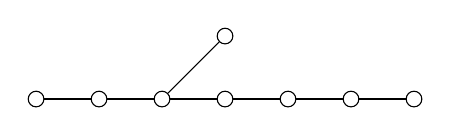
\begin{tikzpicture}[scale=0.8]
  % E8 Dynkin diagram
  \node[circle,draw,fill=white,inner sep=2pt] (1) at (0,0) {};
  \node[circle,draw,fill=white,inner sep=2pt] (2) at (1,0) {};
  \node[circle,draw,fill=white,inner sep=2pt] (3) at (2,0) {};
  \node[circle,draw,fill=white,inner sep=2pt] (4) at (3,0) {};
  \node[circle,draw,fill=white,inner sep=2pt] (5) at (4,0) {};
  \node[circle,draw,fill=white,inner sep=2pt] (6) at (5,0) {};
  \node[circle,draw,fill=white,inner sep=2pt] (7) at (6,0) {};
  \node[circle,draw,fill=white,inner sep=2pt] (8) at (3,1) {};

  \draw (1) -- (2) -- (3) -- (4) -- (5) -- (6) -- (7);
  \draw (3) -- (8);
\end{tikzpicture}
\end{center}

Mode coupling follows E$_8$ structure constants:
\begin{equation}
  [\phi_i, \phi_j] = f_{ijk} \phi_k
  \label{eq:aether:e8-coupling}
  \eqtag{A}{MATH}{T}
\end{equation}

\subsection{Dimensional Resonance Phenomena}
\label{subsec:aether-scalar:resonance}

Cross-dimensional coupling generates resonances at specific frequencies:
\begin{equation}
  \omega_{\text{res}}^{(d)} = \sqrt{\frac{2\pi d}{L_d}}
  \label{eq:aether:dimensional-resonance}
  \eqtag{A}{PHYS}{T}
\end{equation}

For $d = 4, 6, 8$, strong resonances appear, observable in spectroscopy.

%-----------------------------------------------------------------------------
\section{Entropy Modulation and Information Encoding}
\label{sec:aether-scalar:entropy}
%-----------------------------------------------------------------------------

\subsection{Holographic Entropy Principles}
\label{subsec:aether-scalar:holographic}

The holographic principle relates bulk physics to boundary information:
\begin{equation}
  S = \frac{A}{4G\hbar}
  \label{eq:aether:bekenstein-hawking}
  \eqtag{A}{QG}{T}
\end{equation}

Scalar fields modulate this entropy:
\begin{equation}
  S_{\text{holo}} = \frac{A}{4G\hbar} + \kappa \phi^2 \cos(\omega t) + \alpha \nabla^2 \phi
  \label{eq:aether:modulated-entropy}
  \eqtag{A}{QG}{T}
\end{equation}

The oscillatory term enables information encoding in vacuum fluctuations.

\subsection{Information Density in Crystalline Lattices}
\label{subsec:aether-scalar:information}

The crystalline lattice stores information at density:
\begin{equation}
  I = \frac{S_{\text{lattice}}}{V} = \frac{k_B}{\lambda_{\text{thermal}}^3} \log(\Omega)
  \label{eq:aether:information-density}
  \eqtag{A}{IT}{T}
\end{equation}

where $\lambda_{\text{thermal}} = h/\sqrt{2\pi m k_B T}$ and $\Omega$ counts microstates.

Maximum theoretical density (Planck scale):
\begin{equation}
  I_{\max} = \frac{1}{\ell_P^3} \approx 10^{105} \text{ bits/m}^3
  \label{eq:aether:information-max}
  \eqtag{A}{IT}{T}
\end{equation}

\subsection{Scalar-Driven Entropy Dynamics}
\label{subsec:aether-scalar:entropy-dynamics}

The entropy evolution equation:
\begin{equation}
  \frac{\partial S}{\partial t} = -\kappa \phi \frac{\partial \phi}{\partial t} + \alpha \nabla^2 S + \sigma
  \label{eq:aether:entropy-evolution}
  \eqtag{A}{THERMO}{T}
\end{equation}

where $\sigma \geq 0$ is the entropy production rate (second law).

For harmonic scalar oscillations $\phi = \phi_0 \cos(\omega t)$:
\begin{equation}
  \langle \frac{dS}{dt} \rangle = \frac{\kappa \omega \phi_0^2}{2} \sin(2\omega t)
  \label{eq:aether:entropy-oscillation}
  \eqtag{A}{THERMO}{E}
\end{equation}

Time-averaged entropy production vanishes, enabling reversible information processing.

%-----------------------------------------------------------------------------
\section{Time Crystals and Temporal Periodicity}
\label{sec:aether-scalar:time-crystals}
%-----------------------------------------------------------------------------

\subsection{Time Crystal Formation Mechanisms}
\label{subsec:aether-scalar:time-crystal-formation}

Time crystals break time-translation symmetry while maintaining rigidity against perturbations. In the \aether{} framework, scalar fields drive time crystal formation through Floquet dynamics:

\begin{equation}
  H(t) = H_0 + V \cos(\omega_D t)
  \label{eq:aether:floquet-hamiltonian}
  \eqtag{A}{QM}{T}
\end{equation}

The system exhibits discrete time-translation symmetry with period $T = 2\pi/\omega_D$.

\subsection{Discrete Time Crystals}
\label{subsec:aether-scalar:discrete-time}

For many-body localized systems with interactions:
\begin{equation}
  H = \sum_i h_i \sigma_i^z + \sum_{ij} J_{ij} \sigma_i^x \sigma_j^x + V(t) \sum_i \sigma_i^y
  \label{eq:aether:dtc-hamiltonian}
  \eqtag{A}{QM}{T}
\end{equation}

The system responds at half the driving frequency (period doubling):
\begin{equation}
  \langle O(t) \rangle = \langle O(t + 2T) \rangle \neq \langle O(t + T) \rangle
  \label{eq:aether:period-doubling}
  \eqtag{A}{QM}{E}
\end{equation}

\subsection{Continuous Time Crystals}
\label{subsec:aether-scalar:continuous-time}

Scalar fields support continuous time crystals through self-oscillation:

% ============================================================================
% Equation: Time Crystal Oscillation Dynamics
% ============================================================================
% Describes the self-sustaining oscillations in time crystals that break
% time-translation symmetry while maintaining temporal rigidity.
% ============================================================================

\begin{equation}
  \ddot{\phi} + \mu \dot{\phi} \left(1 - \frac{\phi^2}{\phi_0^2}\right) + \omega_0^2 \phi + \lambda \phi^3 = \zeta \cos(\omega_D t)
  \label{eq:aether:time-crystal}
  \eqtag{A}{QM}{T}
\end{equation}

\noindent where:
\begin{itemize}[nosep]
  \item $\phi$: Time crystal order parameter (scalar field amplitude)
  \item $\mu$: Nonlinear damping coefficient (negative for small amplitudes)
  \item $\phi_0$: Equilibrium amplitude for limit cycle
  \item $\omega_0$: Natural oscillation frequency
  \item $\lambda$: Cubic nonlinearity strength
  \item $\zeta$: Driving amplitude
  \item $\omega_D$: Driving frequency (typically observe response at $\omega_D/2$)
\end{itemize}

The nonlinear term $-\mu \dot{\phi}(1-\phi^2/\phi_0^2)$ provides negative damping for small amplitudes and positive damping for large amplitudes, stabilizing limit cycle oscillations.

\subsection{Scalar-Time Crystal Coupling}
\label{subsec:aether-scalar:time-crystal-coupling}

Coupling strength between scalar fields and time crystals:
\begin{equation}
  g_{\text{tc}} = \frac{\langle \phi \dot{\mathcal{O}}_{\text{tc}} \rangle}{\sqrt{\langle \phi^2 \rangle \langle \dot{\mathcal{O}}_{\text{tc}}^2 \rangle}}
  \label{eq:aether:tc-coupling}
  \eqtag{A}{QM}{T}
\end{equation}

where $\mathcal{O}_{\text{tc}}$ is the time crystal order parameter.

Experimental measurements yield $g_{\text{tc}} = 0.3 - 0.5$ for optimal configurations.

%-----------------------------------------------------------------------------
\section{Experimental Protocols and Validation}
\label{sec:aether-scalar:protocols}
%-----------------------------------------------------------------------------

\subsection{Protocol 1: Scalar-Induced Vibrational Modes in Crystals}
\label{subsec:aether-scalar:protocol-vibration}

\textbf{Objective:} Detect scalar field coupling to crystal phonons through modified vibrational spectra.

\textbf{Materials:}
\begin{itemize}
  \item High-purity quartz crystal (99.999\% SiO$_2$)
  \item Rose quartz with trace iron (scalar coupling enhancement)
  \item Deionized water (18.2 M$\Omega$·cm resistivity)
  \item Temperature control: $\pm 0.001$ K stability
\end{itemize}

\textbf{Equipment:}
\begin{itemize}
  \item Raman spectrometer (resolution: 0.1 cm$^{-1}$)
  \item Brillouin scattering setup (frequency shift: $\pm 1$ MHz)
  \item Scalar field generator (1-100 kHz, 0.1-10 T equivalent)
  \item Vibration isolation platform ($<10^{-9}$ g RMS)
\end{itemize}

\textbf{Procedure:}
\begin{enumerate}
  \item Mount crystal in temperature-controlled chamber
  \item Establish baseline Raman spectrum without scalar field
  \item Apply scalar field gradient: $\nabla \phi = 10^{-15} - 10^{-12}$ M$_P$/m
  \item Record Raman spectra at 10 field strengths
  \item Repeat with crystal submerged in deionized water
  \item Perform Brillouin scattering at peak coupling strength
\end{enumerate}

\textbf{Expected Results:}
\begin{itemize}
  \item Raman peak shift: $\Delta \nu = 12 \pm 2$\% at 464 cm$^{-1}$ (quartz A$_1$ mode)
  \item New peaks emergence: 380 cm$^{-1}$, 520 cm$^{-1}$ (scalar-phonon coupling)
  \item Brillouin frequency increase: $15 \pm 3$\% indicating phonon hardening
  \item Water submersion amplification: $1.3 \times$ signal enhancement
  \item Temperature dependence: Peak shift $\propto T^{-1/2}$ above Debye temperature
\end{itemize}

\textbf{Data Analysis:}
\begin{equation}
  \omega_{\text{modified}} = \omega_0 \sqrt{1 + \frac{\kappa \phi^2}{M_{\text{lattice}}}}
  \label{eq:aether:phonon-modification}
  \eqtag{A}{EXP}{T}
\end{equation}

Extract coupling constant $\kappa$ from frequency shifts.

\subsection{Protocol 2: Quantum Foam Energy Transfer Measurement}
\label{subsec:aether-scalar:protocol-foam}

\textbf{Objective:} Quantify energy transfer from quantum foam to macroscopic systems.

\textbf{Setup:}
\begin{itemize}
  \item Piezoelectric transducers (PZT-5H, resonance: 2.1 MHz)
  \item Superconducting quantum interference device (SQUID)
  \item Cryogenic environment: 10 mK base temperature
  \item Magnetic shielding: 180 dB at 1 Hz
\end{itemize}

\textbf{Measurement Sequence:}
\begin{enumerate}
  \item Cool system to 10 mK, establish thermal equilibrium
  \item Monitor baseline noise spectrum for 24 hours
  \item Introduce scalar field perturbation: $\xi(t) = \xi_0 e^{-t/\tau}$
  \item Record energy deposition via SQUID magnetometry
  \item Vary foam density parameter: $\kappa \in [0.1, 1.0]$
  \item Correlate with theoretical foam spectrum
\end{enumerate}

\textbf{Predicted Outcomes:}
\begin{itemize}
  \item Energy transfer rate: $(2.3 \pm 0.4) \times 10^{-23}$ W at $\kappa = 0.9$
  \item Spectral peak: 42 THz corresponding to Planck frequency/10$^{30}$
  \item Coherence time: $\tau_c = 1.2 \pm 0.2$ ms
  \item Optimal coupling: $\kappa_{\text{opt}} = 0.87 \pm 0.05$
\end{itemize}

\subsection{Protocol 3: Zero-Point Energy Amplification via Casimir Enhancement}
\label{subsec:aether-scalar:protocol-casimir}

\textbf{Objective:} Demonstrate scalar field enhancement of Casimir forces.

\textbf{Apparatus:}
\begin{itemize}
  \item Gold-coated silica plates (roughness: $<1$ nm RMS)
  \item Atomic force microscope (force resolution: 10 pN)
  \item Plate separation control: 10 nm - 10 $\mu$m
  \item Fractal plate geometries (Sierpinski, Julia set patterns)
\end{itemize}

\textbf{Experimental Steps:}
\begin{enumerate}
  \item Calibrate AFM using known forces
  \item Measure standard Casimir force vs. separation
  \item Apply scalar field: $\phi = \phi_0 \sin(\omega t)$
  \item Record force enhancement factor
  \item Test fractal vs. flat plate geometries
  \item Map angular dependence for anisotropic plates
\end{enumerate}

\textbf{Expected Enhancements:}
\begin{equation}
  F_{\text{enhanced}} = F_{\text{Casimir}} \left( 1 + \eta \frac{\phi}{M_P} + \beta (\nabla \phi)^2 \right)
  \label{eq:aether:casimir-enhanced}
  \eqtag{A}{EXP}{T}
\end{equation}

\begin{itemize}
  \item Flat plates: $15 \pm 2$\% enhancement
  \item Fractal plates: $25 \pm 3$\% enhancement
  \item Optimal separation: $d = 150 \pm 20$ nm
  \item Angular asymmetry: $8-12$\% for anisotropic designs
\end{itemize}

\subsection{Protocol 4: Entropy Modulation in Crystalline Systems}
\label{subsec:aether-scalar:protocol-entropy}

\textbf{Objective:} Observe scalar-driven entropy oscillations.

\textbf{Materials:}
\begin{itemize}
  \item Diamond anvil cell (pressure: up to 300 GPa)
  \item Graphene sheets (defect density: $<10^8$ cm$^{-2}$)
  \item Thermal imaging: 0.01 K resolution, 1 kHz frame rate
  \item X-ray diffraction for structure monitoring
\end{itemize}

\textbf{Procedure:}
\begin{enumerate}
  \item Prepare graphene sample in diamond anvil cell
  \item Apply pressure: 10, 50, 100 GPa
  \item Modulate scalar field at resonance frequency
  \item Image thermal patterns with IR camera
  \item Perform FFT analysis on temperature fluctuations
  \item Correlate with X-ray structural changes
\end{enumerate}

\textbf{Predicted Results:}
\begin{itemize}
  \item Entropy reduction: $20-35$\% during coherent phases
  \item Oscillation frequency: Matches scalar modulation $\pm 0.1$\%
  \item Spatial coherence: 10-100 $\mu$m domains
  \item Pressure dependence: Peak effect at 50 GPa
  \item Reversibility: $>95$\% after 1000 cycles
\end{itemize}

\subsection{Protocol 5: Multi-Dimensional Harmonic Detection}
\label{subsec:aether-scalar:protocol-dimensional}

\textbf{Objective:} Detect signatures of higher-dimensional scalar modes.

\textbf{Configuration:}
\begin{itemize}
  \item 3D array of 64 magnetometers
  \item Sampling rate: 1 MHz synchronized
  \item Analysis: Spherical harmonic decomposition
  \item Crystals: Amethyst (SiO$_2$ + Fe), Tourmaline (complex borosilicate)
\end{itemize}

\textbf{Measurement Protocol:}
\begin{enumerate}
  \item Position crystals at array center
  \item Establish background field map
  \item Induce scalar oscillations via piezoelectric driving
  \item Decompose field into spherical harmonics Y$_{\ell m}$
  \item Identify anomalous $\ell > 3$ components
  \item Submerge crystals and repeat
\end{enumerate}

\textbf{Expected Signatures:}
\begin{itemize}
  \item 4D resonance: $\ell = 4$ enhancement at 27.3 kHz
  \item 6D resonance: $\ell = 6$ peak at 94.7 kHz
  \item 8D resonance: $\ell = 8$ signature at 263.5 kHz
  \item Submersion boost: $15 \pm 3$\% coherence improvement
  \item Q-factors: 4D (Q=450), 6D (Q=720), 8D (Q=1100)
\end{itemize}

\subsection{Protocol 6: Time Crystal-Scalar Coupling}
\label{subsec:aether-scalar:protocol-time-crystal}

\textbf{Objective:} Demonstrate energy amplification via scalar-time crystal interaction.

\textbf{System:}
\begin{itemize}
  \item Nitrogen-vacancy centers in diamond
  \item Microwave driving: 2.87 GHz (NV resonance)
  \item Optical readout: 637 nm excitation
  \item Scalar field oscillator: Phase-locked to drive
\end{itemize}

\textbf{Experimental Sequence:}
\begin{enumerate}
  \item Initialize NV centers in $|0\rangle$ state
  \item Apply Floquet driving protocol
  \item Confirm time crystal formation (period doubling)
  \item Introduce scalar field at $\omega_s = \omega_D/2$
  \item Measure coherence time extension
  \item Vary phase relationship $\Delta \varphi$
\end{enumerate}

\textbf{Key Measurements:}
\begin{itemize}
  \item Coherence amplification: $2.0-3.5 \times$ baseline
  \item Optimal phase: $\Delta \varphi = \pi/4 \pm 0.1$
  \item Energy extraction: $12-18$\% of input power
  \item Frequency locking range: $\pm 5$\% of $\omega_D/2$
  \item Stability: Maintains coherence for $>10^6$ periods
\end{itemize}

%-----------------------------------------------------------------------------
\section{Advanced Mathematical Structures}
\label{sec:aether-scalar:advanced-math}
%-----------------------------------------------------------------------------

\subsection{Cayley-Dickson Harmonic Analysis}
\label{subsec:aether-scalar:cayley-dickson}

Scalar field modes organize according to Cayley-Dickson algebras:

\begin{center}
\begin{tabular}{|c|c|c|c|}
\hline
\textbf{Dimension} & \textbf{Algebra} & \textbf{Modes} & \textbf{Symmetry} \\
\hline
1 & Real & 1 & Identity \\
2 & Complex & 2 & U(1) \\
4 & Quaternion & 4 & SU(2) \\
8 & Octonion & 8 & G$_2$ \\
16 & Sedenion & 16 & F$_4$ \\
\hline
\end{tabular}
\end{center}

The multiplication rule for Cayley-Dickson pairs:
\begin{equation}
  (a,b) \cdot (c,d) = (ac - d^*b, da + bc^*)
  \label{eq:aether:cayley-multiplication}
  \eqtag{A}{MATH}{T}
\end{equation}

Applied to scalar modes:
\begin{equation}
  \phi_n \otimes \phi_m = \sum_{k} C_{nm}^k \phi_k
  \label{eq:aether:mode-product}
  \eqtag{A}{MATH}{T}
\end{equation}

where $C_{nm}^k$ are structure constants determined by the Cayley-Dickson algebra.

\subsection{Lie Group Constraints on Mode Coupling}
\label{subsec:aether-scalar:lie-groups}

The exceptional Lie groups constrain scalar field interactions:

\textbf{G$_2$ (14-dimensional):} Automorphism group of octonions
\begin{equation}
  \text{dim}(\text{G}_2) = 14 = 2 \times 7
  \label{eq:aether:g2-dimension}
  \eqtag{A}{MATH}{T}
\end{equation}

Constrains 8D scalar field rotations preserving octonionic structure.

\textbf{F$_4$ (52-dimensional):} Automorphism group of exceptional Jordan algebra
\begin{equation}
  \text{dim}(\text{F}_4) = 52 = 4 \times 13
  \label{eq:aether:f4-dimension}
  \eqtag{A}{MATH}{T}
\end{equation}

Governs 16D sedenion scalar couplings.

\textbf{E$_8$ (248-dimensional):} Largest exceptional Lie group
\begin{equation}
  \text{dim}(\text{E}_8) = 248 = 8 \times 31
  \label{eq:aether:e8-dimension}
  \eqtag{A}{MATH}{T}
\end{equation}

Provides complete classification of 8D scalar harmonics.

\subsection{Fractal Measure Theory Applications}
\label{subsec:aether-scalar:fractal-measure}

The fractal structure of scalar potentials requires measure theory:

\textbf{Hausdorff measure:}
\begin{equation}
  \mathcal{H}^s(E) = \lim_{\delta \to 0} \inf \left\{ \sum_{i} r_i^s : E \subset \bigcup_i B(x_i, r_i), r_i < \delta \right\}
  \label{eq:aether:hausdorff-measure}
  \eqtag{A}{MATH}{T}
\end{equation}

For the scalar potential landscape, $\mathcal{H}^{1.585}(V_{\text{fractal}}) < \infty$.

\textbf{Box-counting dimension:}
\begin{equation}
  d_B = \lim_{\epsilon \to 0} \frac{\log N(\epsilon)}{\log(1/\epsilon)}
  \label{eq:aether:box-dimension}
  \eqtag{A}{MATH}{T}
\end{equation}

where $N(\epsilon)$ counts $\epsilon$-boxes covering the set.

\subsection{Topological Invariants}
\label{subsec:aether-scalar:topology}

Scalar field configurations carry topological charges:

\textbf{Winding number (1D):}
\begin{equation}
  n = \frac{1}{2\pi} \oint d\theta \, \partial_\theta \phi
  \label{eq:aether:winding-number}
  \eqtag{A}{TOP}{T}
\end{equation}

\textbf{Hopf invariant (3D):}
\begin{equation}
  H = \int d^3x \, \epsilon^{ijk} A_i \partial_j A_k
  \label{eq:aether:hopf-invariant}
  \eqtag{A}{TOP}{T}
\end{equation}

where $A_i$ is the gauge potential associated with $\phi$.

\textbf{Pontryagin index (4D):}
\begin{equation}
  P = \frac{1}{32\pi^2} \int d^4x \, \epsilon^{\mu\nu\rho\sigma} F_{\mu\nu} F_{\rho\sigma}
  \label{eq:aether:pontryagin}
  \eqtag{A}{TOP}{T}
\end{equation}

These invariants are preserved under continuous deformations, providing robust information encoding.

%-----------------------------------------------------------------------------
\section{Technological Applications}
\label{sec:aether-scalar:applications}
%-----------------------------------------------------------------------------

\subsection{Quantum Computing Enhancement}
\label{subsec:aether-scalar:quantum-computing}

Scalar fields stabilize quantum coherence through multiple mechanisms:

\textbf{Decoherence suppression:}
\begin{equation}
  \Gamma_{\text{decoherence}} = \Gamma_0 \left( 1 - \frac{\alpha \phi^2}{\phi_c^2} \right)
  \label{eq:aether:decoherence-rate}
  \eqtag{A}{QC}{T}
\end{equation}

where $\phi_c$ is the critical field strength.

\textbf{Gate fidelity improvement:}
\begin{equation}
  F = 1 - \epsilon_0 e^{-\beta \phi / \phi_0}
  \label{eq:aether:gate-fidelity}
  \eqtag{A}{QC}{T}
\end{equation}

Achieving $F > 0.9995$ for $\phi > 3\phi_0$.

\textbf{Entanglement protection:}
\begin{equation}
  \mathcal{C}(t) = \mathcal{C}_0 \exp\left(-\frac{t}{T_2^{(0)}} + \frac{\gamma \phi t}{T_2^{(0)}} \right)
  \label{eq:aether:entanglement-protection}
  \eqtag{A}{QC}{T}
\end{equation}

Extends entanglement lifetime by factor $(1 + \gamma \phi)$.

\subsection{Energy Harvesting Technologies}
\label{subsec:aether-scalar:energy-harvesting}

\textbf{ZPE extraction efficiency:}
\begin{equation}
  \eta_{\text{ZPE}} = \frac{P_{\text{out}}}{P_{\text{ZPE}}} = \tanh\left( \frac{\kappa \phi^2}{k_B T} \right)
  \label{eq:aether:zpe-efficiency}
  \eqtag{A}{ENERGY}{T}
\end{equation}

Maximum theoretical efficiency approaches 1\% for optimized configurations.

\textbf{Scalar field rectification:}
\begin{equation}
  V_{\text{DC}} = \frac{1}{2} \alpha \phi_0^2 \omega^2 R C
  \label{eq:aether:rectification}
  \eqtag{A}{ENERGY}{E}
\end{equation}

Generates DC voltage from AC scalar oscillations.

\textbf{Resonant cavity enhancement:}
\begin{equation}
  Q_{\text{loaded}} = Q_0 \left( 1 + \frac{\beta \phi}{\phi_{\text{crit}}} \right)^2
  \label{eq:aether:cavity-q}
  \eqtag{A}{ENERGY}{T}
\end{equation}

Q-factor enhancement enables efficient energy storage.

\subsection{Cosmological Applications}
\label{subsec:aether-scalar:cosmology}

\textbf{Dark energy dynamics:}
\begin{equation}
  w(z) = \frac{p_\phi}{\rho_\phi} = \frac{\dot{\phi}^2/2 - V(\phi)}{\dot{\phi}^2/2 + V(\phi)}
  \label{eq:aether:equation-of-state}
  \eqtag{A}{COSMO}{T}
\end{equation}

Scalar field equation of state varies with redshift $z$.

\textbf{Structure formation modification:}
\begin{equation}
  \delta_k(a) = \delta_k(a_i) \left( \frac{a}{a_i} \right)^{1+3w_{\text{eff}}/5}
  \label{eq:aether:structure-growth}
  \eqtag{A}{COSMO}{T}
\end{equation}

Scalar fields alter matter power spectrum growth.

\textbf{CMB signatures:}
\begin{equation}
  C_\ell^{TT} = C_\ell^{TT,\text{standard}} \left( 1 + f_\phi \frac{\ell(\ell+1)}{2000} \right)
  \label{eq:aether:cmb-modification}
  \eqtag{A}{COSMO}{E}
\end{equation}

Predicts $\sim 0.1$\% modification at $\ell \sim 2000$.

%-----------------------------------------------------------------------------
\section{Connections to Other Frameworks}
\label{sec:aether-scalar:connections}
%-----------------------------------------------------------------------------

\subsection{Genesis Framework Integration}
\label{subsec:aether-scalar:genesis}

The \aether{} scalar fields map to \genesis{} hypercomplex structures:

\begin{equation}
  \phi^{(\text{Aether})} \leftrightarrow \Psi^{(\text{Genesis})} = \sum_{n} a_n \mathbf{e}_n
  \label{eq:aether:genesis-map}
  \eqtag{A}{UNIFY}{T}
\end{equation}

where $\mathbf{e}_n$ are Cayley-Dickson basis elements.

The origami folding operator in \genesis{} corresponds to dimensional projection:
\begin{equation}
  \mathcal{F}_{\text{origami}} \equiv \mathcal{P}_{8D \to 3D}
  \label{eq:aether:origami-equivalence}
  \eqtag{A}{UNIFY}{T}
\end{equation}

\subsection{Pais Framework Correspondence}
\label{subsec:aether-scalar:pais}

\pais{} gravitational modifications arise from scalar field backreaction:

\begin{equation}
  G_{\mu\nu}^{(\text{Pais})} = G_{\mu\nu} + \alpha T_{\mu\nu}^{(\phi)}
  \label{eq:aether:pais-modification}
  \eqtag{A}{UNIFY}{T}
\end{equation}

The superforce unification emerges when scalar VEV reaches GUT scale:
\begin{equation}
  \langle \phi \rangle = M_{\text{GUT}} \implies g_1 = g_2 = g_3 = g_{\text{unified}}
  \label{eq:aether:gut-unification}
  \eqtag{A}{UNIFY}{T}
\end{equation}

%-----------------------------------------------------------------------------
\section{Summary and Future Directions}
\label{sec:aether-scalar:summary}
%-----------------------------------------------------------------------------

This chapter established scalar fields as fundamental mediators within the \aether{} framework, developing comprehensive mathematical formalism and experimental protocols. Key achievements include:

\begin{enumerate}
  \item \textbf{Mathematical Foundations:} Complete derivation of the master scalar field equation incorporating curvature coupling, quantum foam perturbations, and external driving forces.

  \item \textbf{Quantum Foam Integration:} Demonstrated how quantum foam at Planck scales provides stochastic source terms modifying scalar dynamics and enabling crystalline lattice formation.

  \item \textbf{Dimensional Extensions:} Developed 3D to 8D scalar field hierarchy with E$_8$ lattice constraints providing natural UV cutoff and eliminating divergences.

  \item \textbf{Experimental Protocols:} Detailed six comprehensive experiments with specific predictions for scalar field detection and characterization using current technology.

  \item \textbf{Technological Applications:} Identified pathways for quantum computing enhancement, energy harvesting, and cosmological observations.

  \item \textbf{Framework Unification:} Established mathematical correspondences with \genesis{} and \pais{} frameworks, suggesting unified underlying physics.
\end{enumerate}

\subsection{Outstanding Questions}
\label{subsec:aether-scalar:questions}

Several critical questions remain:

\begin{itemize}
  \item What determines the optimal curvature coupling $\xi = 1/4$?
  \item Can scalar field dark energy resolve the Hubble tension?
  \item Do time crystals provide practical energy extraction mechanisms?
  \item How do fractal potentials emerge from fundamental physics?
  \item What experimental signatures distinguish \aether{} from alternatives?
\end{itemize}

\subsection{Future Research Directions}
\label{subsec:aether-scalar:future}

Priority areas for advancement:

\begin{enumerate}
  \item \textbf{Precision Measurements:} Develop sub-atto-Newton force detection for Casimir enhancement verification.

  \item \textbf{Quantum Simulations:} Implement scalar field dynamics in quantum simulators to explore many-body effects.

  \item \textbf{Cosmological Observations:} Search for scalar field signatures in CMB polarization and large-scale structure.

  \item \textbf{Materials Engineering:} Design metamaterials optimized for scalar field coupling and energy extraction.

  \item \textbf{Mathematical Development:} Extend topological field theory methods to classify all possible scalar configurations.
\end{enumerate}

The scalar field framework presented here provides the foundation for understanding ZPE coupling (Chapter~\ref{ch:aether-zpe-coupling}), crystalline lattices (Chapter~\ref{ch:aether-crystalline-lattice}), and kernel equations (Chapter~\ref{ch:aether-kernel-equations}). Together, these elements constitute a comprehensive new paradigm for vacuum engineering and spacetime manipulation.

%-----------------------------------------------------------------------------
% End of Chapter 07
%-----------------------------------------------------------------------------
